 \documentclass[12pt]{article}
\pagestyle{myheadings}


%Enter your name, the portfolio problem number, and the draft number.
\title{Agujeros negros de Kerr}
\author{Matías Borghi}

%Enter your name, the portfolio problem number, and the draft number.  This will be a heading on pages after the first page.
\markright{Agujeros negros de Kerr - Matias Borghi}

\usepackage[spanish, es-tabla]{babel}
\usepackage[utf8x]{inputenc}
\usepackage{amsmath}
\usepackage{graphicx}
\usepackage{xcolor}
\usepackage{float}
\usepackage{wrapfig}
\usepackage{tensor}
\usepackage{amsmath,amssymb,amsthm,amsfonts,graphics}
\usepackage{hyperref}
%\hypersetup{
%	linktoc=all,
%    colorlinks=true,
%    linkcolor=blue,
%    filecolor=magenta,      
%    urlcolor=cyan,
%}

%The following commands allow us to typeset theorems, propositions, definitions, etc.
\theoremstyle{plain}
\newtheorem{theorem}{Theorem}
\newtheorem{lemma}[theorem]{Lemma}
\newtheorem{corollary}[theorem]{Corollary}
\newtheorem{proposition}[theorem]{Proposition}
\newtheorem*{definition}{Definition}

\renewcommand{\qedsymbol}{\ensuremath{\blacksquare}}
\newcommand{\N}{\mathbb{N}}
\newcommand{\Z}{\mathbb{Z}}
\newcommand{\Q}{\mathbb{Q}}
\newcommand{\R}{\mathbb{R}}


\begin{document}
\maketitle

%Enter your email address.
\begin{center}
\textbf{borghi.matias@gmail.com}
\end{center}

\tableofcontents
%-----------------INTRODUCCIÓN-----------------------------------
\section{Introducción}
El objetivo de la presente monografía es describir la métrica de Kerr, sus diferencias con la métrica de Schwarzschild y presentar datos observacionales de agujeros negros que sustenten la misma.

Para ello, primero se explicarán conceptos generales de agujeros negros, se introducirá la solución más simple, que es la métrica de Schwarzschild y luego se introducirá la métrica de Kerr.
%------------RESEÑA-HISTORICA-------------------------------------
\section{Reseña histórica}
1915 es un año muy recordado para los físicos por ser el año en que Einstein publicó su Teoría General de la Relatividad. La motivación, aparte de entender las implicancias físicas de su teoría obviamente, era resolver la ecuación que lleva su nombre hoy en día \ref{einseq}. Al año siguiente, en 1916, Karl Schwarzschild proponía la primera solución analítica correspondiente a la solución de vacío para objetos esféricamente simétricos de masa $M$ estáticos. En 1922 Alexander Friedmann desarrolla las ecuaciones que llevan su nombre acerca de la expansión del universo isotrópico y homogéneo. Luego la épocas de guerra provocaron que las mentes más brillantes estuvieran inmersas en el desarrollo de proyectos de bombas atómicas como el Proyecto Manhattan. 

\begin{figure}[H]
\centering
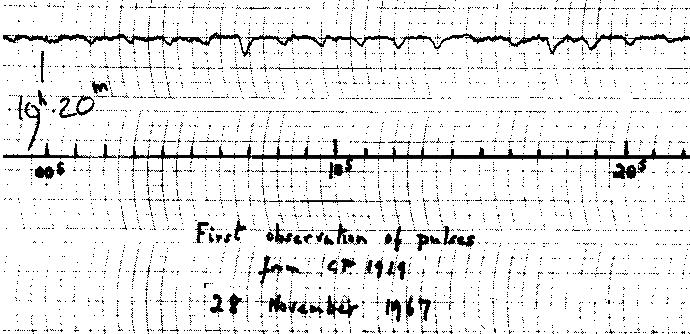
\includegraphics[width=\textwidth]{pulsar.jpg}
\caption{Descubrimiento del primer pulsar en 1967. Muestra original del grabado de la intensidad en función del tiempo.}
\label{pulsar}
\end{figure}

\begin{wrapfigure}{r}{0.5\textwidth}
  \begin{center}
    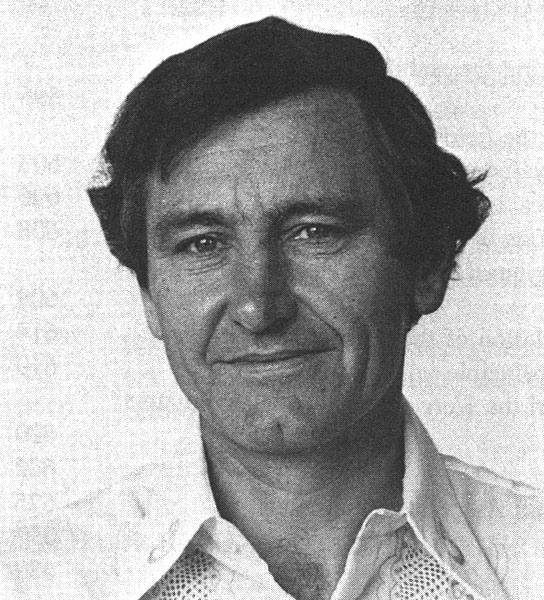
\includegraphics[width=0.48\textwidth]{retrato_kerr.jpg}
  \end{center}
  \caption{Retrato del descubridor de la métrica que lleva su nombre, Roy Kerr.}
\label{foto_kerr}
\end{wrapfigure}

Luego de finalizada la guerra, en los 60's y 70's el interés por el estudio de la relatividad general o más específicamente en los agujeros negros floreció debido al desarrollo de nuevas herramientas matemáticas e instrumentos astronómicos así como también el descubrimiento de objetos como los púlsares en 1967 \ref{pulsar}, en una etapa conocida como la \textbf{época de oro de la astrofísica relativista}. Las soluciones a las ecuaciones de Einstein ya no eran vistas como meras soluciones matemáticas sino que ya se disponían de resultados experimentales. En ésta época se formaron nuevos grupos de investigación en relatividad general: en Princeton \textbf{John Archibald Wheeler} que posteriormente creó el término \textit{agujero de gusano} y fue el primer físico en utilizar el nombre \textit{agujero negro} en una conferencia en 1967; en Cambridge \textbf{Dennis Willian Sciama}, conocido como el padre de la cosmología moderna y \textbf{Roger Penrose}; en la Universidad de Moscú \textbf{Yakov Borisov Zel'dovich}, reconocido entre otras cosas por sus investigaciones con discos de acreción y en la Universidad de Hamburgo \textbf{Pascual Jordan}. Por último, pero no menos importante, se creó un grupo en Austin,Texas liderado por \textbf{Alfred Schild}, donde un jóven matemático neo zelandés llamado \textbf{Roy Patrick Kerr} \ref{foto_kerr} se unió en 1962 y, al año siguiente, publicó su investigación de dos hojas llamada \textit{"Gravitational field of a spinning mass as an example of algebraically special metrics"} \cite{kerr_paper}(figura \ref{paper_foto} ) que describe la solución a la ecuación de Einstein en el vacío válida fuera de una masa rotante estacionaria. La importancia física de la misma no fue inmediatamente comprendida. Es por ello que Dennis Sciama le pidió a un estudiante \textbf{Brandon Carter} que investigara la solución obtenida por Kerr. Kerr presentó su trabajo en coordenadas cartesianas las cuales no son muy prácticas. Hoy en día se suelen utilizar las coordenadas de Boyer Lindquist propuestas por \textbf{Robert Boyer} en 1967. Boyer se unió al grupo de Kerr en Austin en los 60's pero murió junto con otras personas al ser victima de un ataque de un estudiante de la marina estadounidense desde la torre de la universidad. 



\begin{figure}[H]
\centering
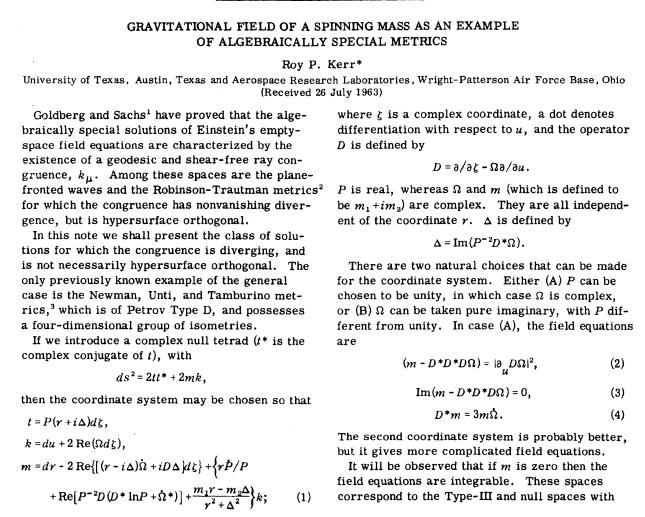
\includegraphics[width=\textwidth]{paper_original.jpeg}
\caption{Paper donde Kerr publicó el descubrimiento titulado "Gravitational field of a spinning mass as an example of algebraically special metrics".}
\label{paper_foto}
\end{figure}

%---------------AGUJERO-NEGRO-------------------------------------
\section{¿Qué es un agujero negro?}
Robert Wald define en su libro \cite{wald} a un agujero negro como una región del espacio-tiempo donde la gravidad que previene que cualquier cosa, inclusive la luz, pueda escapar del mismo. 

\begin{figure}[H]
\centering
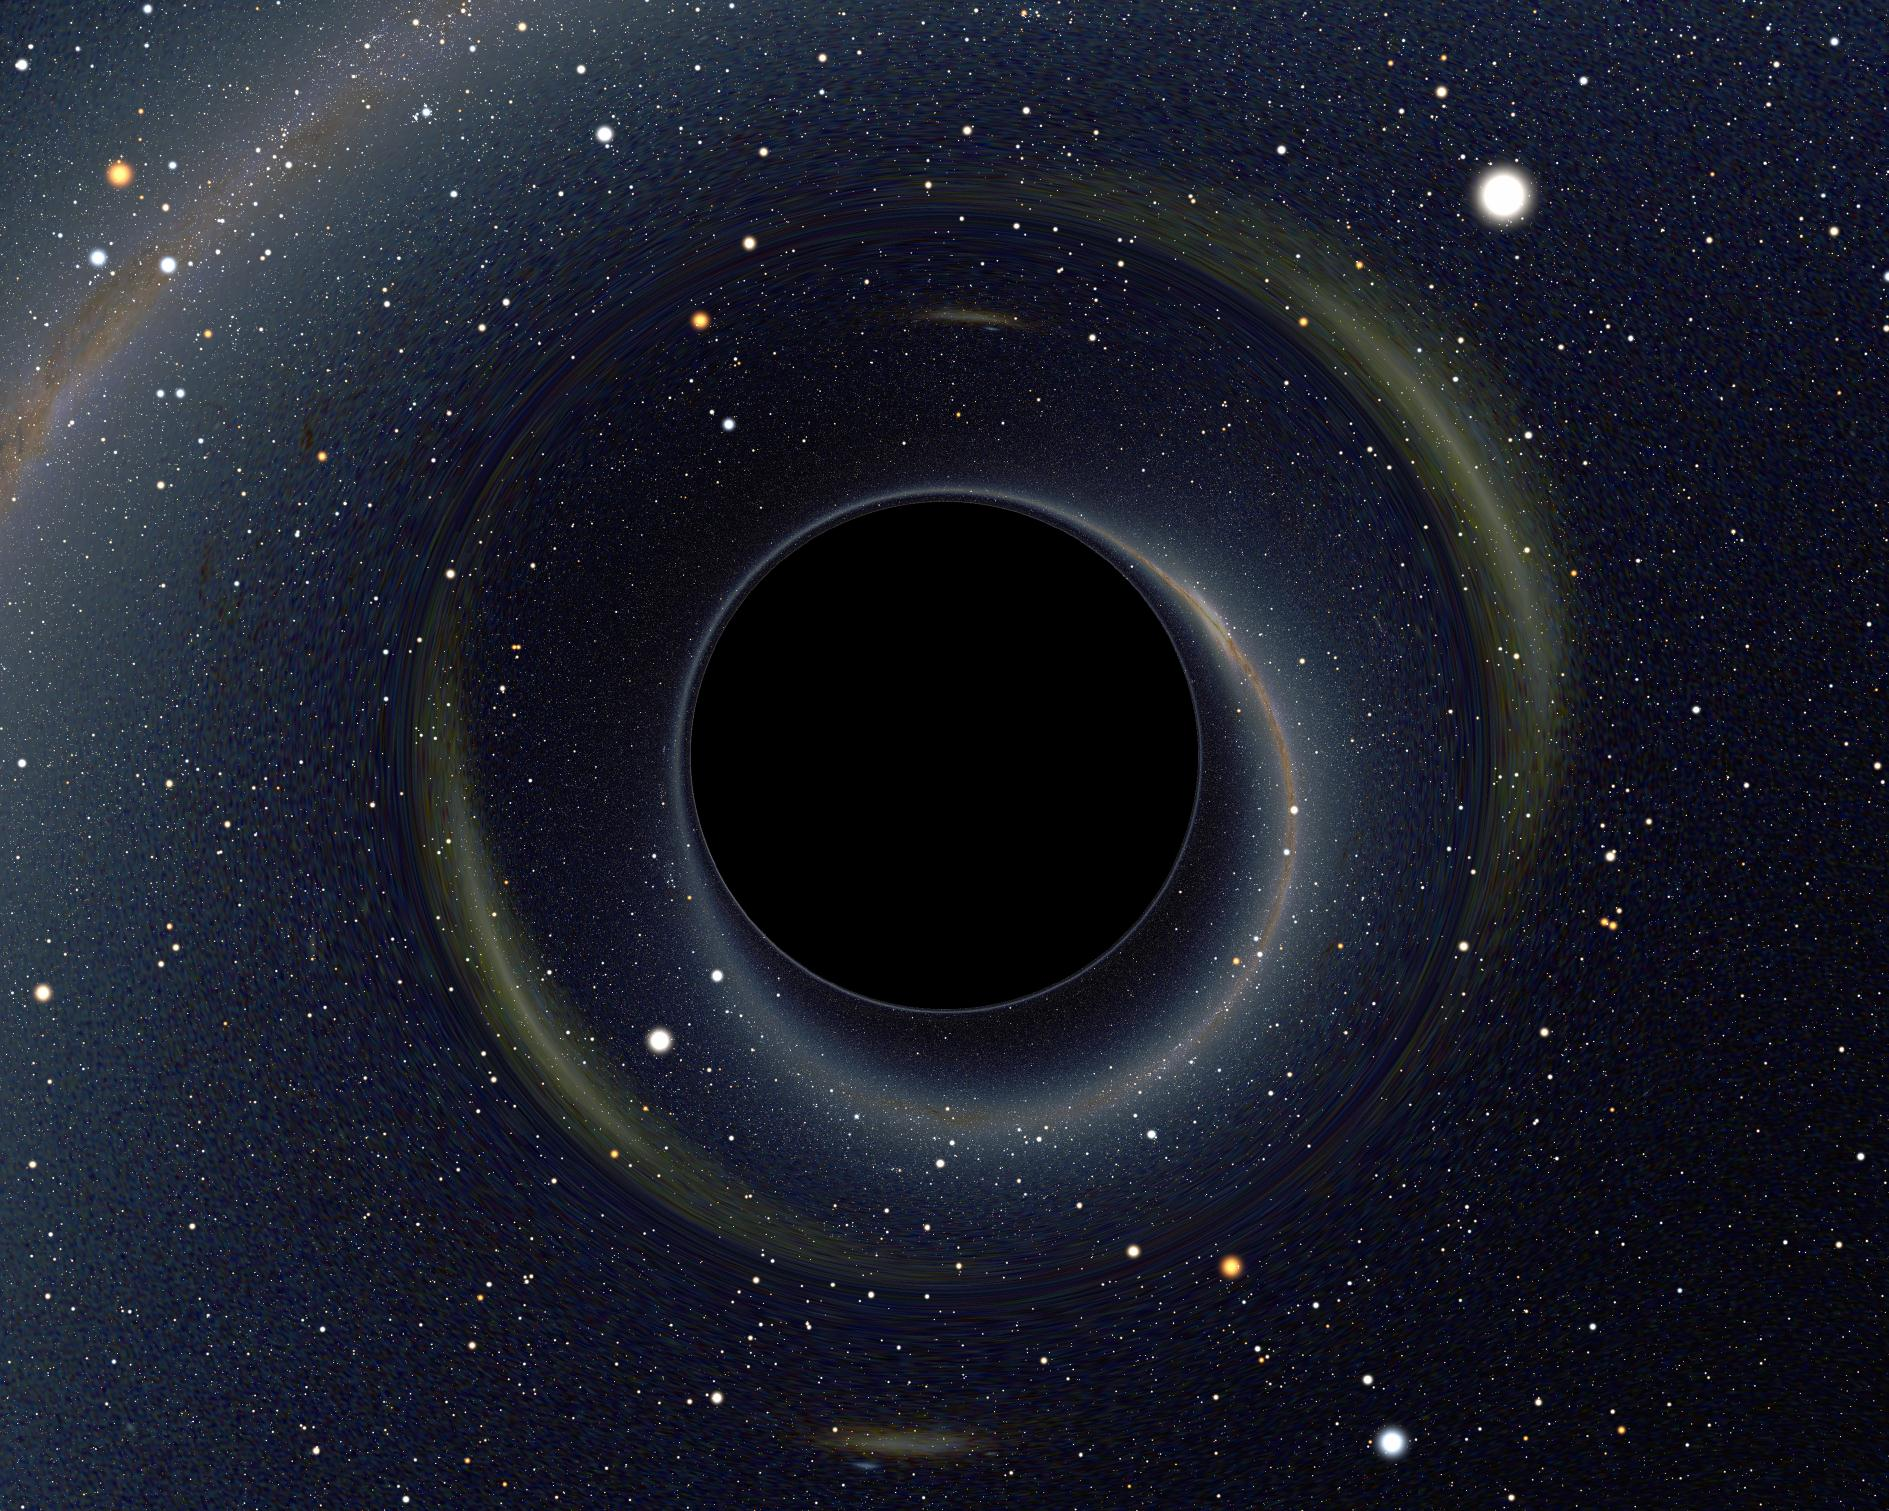
\includegraphics[scale=0.5]{Black_Hole.jpg}
\caption{Imágen ilustrativa de un agujero negro basada en una simulación computacional.}
\label{bh}
\end{figure}

Antes de continuar se enunciará un teorema muy importante llamado teorema de \textit{No-Hair} que dice que en condiciones estables luego de la formación de una agujero negro, éstos tienen tres propiedades físicas independientes: \textbf{masa, carga y momento angular}. Cualquier agujero negro que tenga estos tres parámetros idénticos clásicamente será indistinguible.

De acuerdo a su carga y su momento angular los agujeros negros se pueden clasificar según:
\begin{table}[H]
\centering
\begin{tabular}{ c|c c }
   & $J\,=\,0$ & $J\,\neq\,0$ \\ \hline
  $Q\,=\,0$ & Schwarzschild & Kerr \\ 
   $Q\,\neq\,0$& Reissner-Nordstrom & Kerr-Newmann \\ 
\end{tabular}
\end{table}

mientras que, de acuerdo a su masa, se pueden clasificar como
\begin{itemize}
\item agujeros negros supermasivos con una masa entre $10^5$ y $10^{10}\,M_{\odot}$,
\item agujeros negros intermedios con una masa de $10^3\,M_{\odot}$,
\item agujeros negros estelares con una masa de $10\,M_{\odot}$,
\item micro agujeros negros con una masa aproximada correspondiente a la masa de la luna.
\end{itemize}
%--------METRICA-DE-SCHWARZSCHILD---------------------------------
\section{Métrica de Schwarzschild}
A continuación se presentarán brevemente los resultados que nos interesan acerca de la métrica de Schwarzaschild para luego ser comparados con los de Kerr.

El \textit{teorema de Birkhoff} dice que la única solución posible exterior en el vacío esféricamente simétrica de las ecuaciones de Einstein es la solución de Schwarzschild. La misma escrita en coordenadas esféricas es

\begin{flalign}\label{schwarmetric}
&ds^2\,=\,\left(1-\frac{2Gm}{rc^2}\right)c^2dt^2-\left(1-\frac{2Gm}{rc^2}\right)^{-1}dr^2-r^2d\Omega ^2,&  \\ \nonumber \\ \nonumber
 &\text{donde } d\Omega ^2\,=\,d\theta ^2+\sin ^2\theta d\phi ^2.&
\end{flalign}

\subsection{Singularidades}
En un principio se sospechaba (\textit{Lifshitz et. al.}) que las singularidades aparecían por simetrías de la teoría y que por ende no aparecerían en soluciones generales. Pero Penrose y Hawking \cite{ph_sing} demostraron a fines de los 60s que las singularidades sí aparecían genéricamente.

Las singularidades de la métrica se definen como los puntos donde la métrica diverge. Trivialmente la métrica de Schwarzschild diverge para $r=0$ y $r_s=2GM/c^2$. Éste último es conocido como el radio de Schwarzschild y tiene la particularidad de que es una singularidad aparente. Es decir, que ante un cambio de coordenadas la misma ya no lo es. El cambio de coordenadas en cuestión es el de Eddington-Finkelstein. La metrica se lleva a la forma

\begin{flalign}\label{schwaref}
&ds^2\,=\,\left(1-\frac{2Gm}{rc^2}\right)(c^2dt^2-dr_*^2)-r^2d\Omega ^2,&  \\ \nonumber \\ \nonumber
 &\text{donde } d\Omega ^2\,=\,d\theta ^2+\sin ^2\theta d\phi ^2 & \\ \nonumber \\ \nonumber
 &\text{y } r_*\,=\,r+\frac{2GM}{c^2}\log \left(\frac{r-2GM/c^2}{2GM/c^2}\right).
\end{flalign}

Otra manera de determinar que $r_s$ no es una singularidad esencial es a través del escalar de Kretschmann. Éste es un invariante que diverge en las mismas coordenadas que las singularidades esenciales y se calcula como la contracción de los cuatro componentes del tensor de curvatura,
\begin{flalign}
&K=R^{\mu \nu \sigma \rho}R_{\mu \nu \sigma \rho}\,=\,\frac{12r_s^2}{r^6}\,=\,\frac{48G^2M^2}{c^4r^6}.&
\end{flalign}

\subsection{Horizonte de eventos}
La hipersuperficie determinada por $r = r_s$ se llama horizonte de eventos. Esto significa que un fotón (o cualquier partícula masiva) necesitará inifinita cantidad de energía para poder escapar hacia el exterior de la superficie si se encuentra dentro. Es por ello que eventos que ocurren en $r<r_s$ están desconectados del resto del universo.

En la figura \ref{schwar_cone} se muestra un diagrama del espacio tiempo en coordenadas de Eddington-Finkelstein. En coordenadas esféricas no es conveniente realizar el gráfico por la singularidad en $r_s$. Notar que los fotones en el horizonte de eventos no tienen manera de escapar ya que su dirección es paralela al mismo. Toda partícula que ingrese dentro de la superficie terminará en la singularidad $r=0$. 

\begin{figure}[H]
\centering
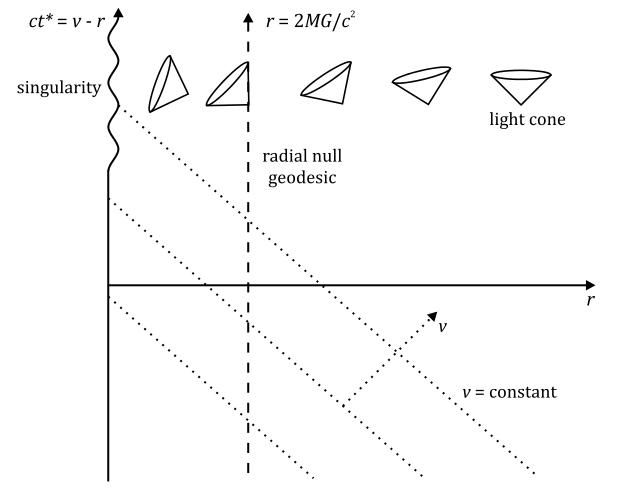
\includegraphics[width=0.75\textwidth]{schwar_cone.JPG}
\caption{Diagrama del espacio tiempo para la métrica de Schwarzschild en coordenadas de Eddington Finkelstein mostrando los conos de luz. $r=r_s$ es el radio de Schwarzschild donde está ubicado el horizonte de eventos.}
\label{schwar_cone}
\end{figure}

%--------METRICA-DE-KERR------------------------------------------
\section{Métrica de Kerr}
A continuación se analizará la métrica de Kerr, objetivo principal de la ésta monografía.
%--------METRICA-DE-KERR-SCHILD-----------------------------------
\subsection{Métrica de Kerr-Schild}
La ecuación \ref{kerrschild} es la forma de la métrica publicada por Kerr en 1963 (ver figura \ref{paper_foto} ). La misma está en coordenadas cartesianas y no es la forma más ampliamente usada. 
\begin{equation}\label{kerrschild}
\begin{split}
ds^2\,&=\,c^2d\hat{t}^2-dx^2-dy^2-dz^2-\frac{2\mu r^3}{r^4+a^2z^2}\\ 
&\times \left[ cd\hat{t}^2-\frac{r}{r^2+a^2}(xdx+ydy)-\frac{a}{r^2+a^2}(xdy-ydx)-\frac{z}{r}dz  \right]^2
\end{split}
\end{equation}
Haciendo una transformación de coordenadas como se muestra a continuación se obtiene la métrica de Kerr en coordenadas de Boyer- Lindquist \ref{boylind} que, a diferencia de las de Kerr-Schild, es más práctica. Es por ello que no se explicarán los términos y los parámetros en detalle y se dejarán para la sección siguiente.
\begin{flalign}\nonumber
&cd\hat{t} = cdt- 2\mu r/\Delta dr,& \\ \nonumber
&x = (r\cos \phi '+a\sin \phi') \sin \theta ,& \\ \nonumber
&y = (r\sin \phi '-a\cos \phi') \sin \theta ,& \\ \nonumber
&z = r\cos \theta ,&\\ \nonumber
&\text{donde } d\phi '=d\phi- (a/\Delta )dr.&
\end{flalign}

%--------------COORDENADAS-BOYER-LINDQUIST------------------------
\subsection{Métrica en coordenadas de Boyer - Lindquist}\label{boylind}
Como se explicó en la sección anterior la métrica de Kerr es ampliamente utilizada en coordenadas de Boyer-Lindquist. Esto es debido al número de términos diagonales que posee es mínimo. Por un lado la métrica de Boyer-Lindquist tiene un único término diagonal, por el otro Kerr-Schild posee tres términos no diagonales. 
\begin{flalign} \label{bymetric}
ds^2\,&=\,c^2\left(1-\frac{2\mu r}{\rho ^2}\right)dt^2+\frac{4\mu acr\sin ^2\theta}{\rho ^2}dtd\phi -\frac{\rho ^2}{\Delta}dr^2-\rho ^2 d\theta ^2& \\ \nonumber \\ \nonumber
&-\left( r^2 + a^2+\frac{2\mu ra^2\sin ^2\theta}{\rho ^2} \right) \sin ^2\theta d\phi ^2,&
\end{flalign}
donde  $\mu = GM/c^2$ y $a=J/Mc$ son constantes, $M$ es la masa del agujero negro, $G$ es la constante de gravitación, $c$ es la velocidad de la luz en el vacíoy $J$ es el momento angular del agujero negro. A su vez los parámetros $\rho$ y $\Delta$ están definidos como:
\begin{flalign}\nonumber
&\rho ^2 = r^2+a^2 \cos ^2\theta&  \\ \nonumber
&\Delta = r^2-2\mu r+a^2&
\end{flalign}
La ecuación \ref{bymetric} se puede reescribir haciendo la sustitución: $\Sigma ^2 = (r^2+a^2)^2-a^2\Delta\sin ^2\theta$ con un término de rotación $\omega$ del agujero negro escrito en forma explícita como se muestra en la ecuación \ref{bymetric2} .
\begin{flalign} \label{bymetric2}
ds^2&=\frac{\Delta -a^2\sin ^2\theta}{\rho ^2}c^2dt^2+\frac{4\mu acr\sin ^2\theta}{\rho ^2}dtd\phi -\frac{\rho ^2}{\Delta}dr^2-\rho ^2 d\theta ^2 -\frac{\Sigma ^2\sin ^2\theta}{\rho ^2} d\phi ^2& \\ \nonumber
&= \frac{\rho ^2\Delta}{\Sigma ^2}c^2dt^2 -\frac{\Sigma ^2\sin ^2\theta}{\rho ^2}(d\phi-\omega dt)^2 -\frac{\rho ^2}{\Delta}dr^2-\rho ^2 d\theta ^2.&
\end{flalign}
Con $\displaystyle \omega \,=\, 2\mu cra/\Sigma ^2$.
%%-------------COMPONENTES CONTRAVARIANTES DE LA METRICA---------
\subsection{Componentes contravariantes de la métrica}
Dado que la única componente no diagonal en coordenadas de Boyer-Lindquist es $dtd\phi$ las componentes contravariantes de la métrica para $r$ y $\theta$ se calculan como la inversa. 
\begin{equation}\nonumber
\begin{aligned}
g^{rr} = g_{rr}^{-1}=-\frac{\Delta}{\rho ^2},\hspace{1cm} g^{\theta\theta} = g_{\theta\theta}^{-1}=-\frac{1}{\rho ^2}. 
\end{aligned}
\end{equation}
Mientras que las restantes componentes se calculan diagonalizando la matriz sin los términos anteriormente calculados
\begin{equation}\nonumber
\begin{aligned}
g^{tt} =\frac{\Sigma ^2}{c^2\rho ^2\Delta},\hspace{0.5cm} g^{t\phi} = \frac{2\mu ar}{c\rho ^2\Delta}, \hspace{0.5cm} g^{\phi\phi} = \frac{a^2\sin ^2\theta-\Delta}{\rho ^2\Delta\sin ^2\theta}. 
\end{aligned}
\end{equation}
%-------------TENSOR-DE-RIEMANN----------------------------------
\subsection{Tensor de Riemann}\label{riemann}
El tensor de Riemann o tensor de curvatura se puede calcular en función de las conexiones afines según
\begin{equation}
R^{\rho}_{\sigma\mu\nu}\,=\,\partial_{\mu}\Gamma^{\rho}_{\nu\sigma}-\partial_{\nu}\Gamma^{\rho}_{\mu\sigma}+\Gamma^{\rho}_{\mu\lambda}\Gamma^{\lambda}_{\nu\sigma}-\Gamma^{\rho}_{\nu\lambda}\Gamma^{\lambda}_{\mu\sigma}.
\end{equation}
Para el caso de las coordendas de Boyer-Lindquist en la métrica de Kerr se obtiene
\begin{flalign} \nonumber
&R_{1414}=-R_{2424}=-2R_{3434}=2R_{1212}=2R_{1313}=-R_{2323}=-\frac{2\mu r(r^2-3a^2\cos ^2\theta)}{(r^2+a^2\cos ^2\theta)^3},&\\ 
&R_{2341}=R_{1342}=-R_{1243}=\frac{2\mu a\cos \theta(3r^2-3a^2\cos ^2\theta)}{(r^2+a^2\cos ^2\theta)^3}.&
\end{flalign}
%----------ESCALAR-DE-KRETSCHMANN--------------------------------
\subsection{Escalar de Kretschmann}\label{kretschmann}
El escalar de Kretschmann se define como la contracción del tensor de Riemann \ref{riemann} consigo mismo. Es de vital importancia al estudiar singularidades. Permite distinguir si una singularidad es esencial o evitable por el hecho de que éste escalar diverge para las primeras. Esto es, una singularidad $s$ es esencial $\Leftrightarrow$ $1/K(s)\rightarrow 0$ $\Leftrightarrow$ $K(s) \rightarrow \infty$. Usando los resultados del tensor de curvatura se obtiene que para la metrica de Kerr
\begin{flalign}
&K\,=\,R^{\mu \nu \sigma \rho}R_{\mu \nu \sigma \rho}=\frac{48\mu ^2(r^2-a^2\cos ^2\theta)\left[ (r^2-a^2\cos ^2\theta)^2 -16r^2a^2\cos ^2\theta \right] }{(r^2+a^2\cos ^2\theta)^6}.&
\end{flalign}
%------------------ECUACION-DE-EINSTEIN--------------------------
\subsection{Ecuación de Einstein}
La ecuación de Einstein sin constante cosmológica se muestra en \ref{einseq}.
\begin{equation}\label{einseq}
G_{\mu\nu}\,=\,R_{\mu\nu}-\frac{1}{2}Rg_{\mu\nu} = \frac{8\pi G}{c^4}T_{\mu\nu}, 
\end{equation}
donde
\begin{itemize}
\item $G_{\mu\nu}$ es el tensor de curvatura de Einstein,
\item $R_{\mu\nu}$ es el tensor de curvatura de Ricci calculado como la contracción del tensor de Riemann \ref{riemann} $R_{\mu \nu} = R^{\lambda}_{\mu \lambda \nu}$.
\item $g_{\mu\nu}$ es el tensor métrico,
\item $G\,=\,6.67\times 10^{-11}\,N(m/kg)^2$ es la constante gravitatoria de Newton,
\item $c\,=\,3\times 10^{10}\,m/s$ es la velocidad de la luz en el vacío,
\item $T_{\mu\nu}$ es el tensor energía-impulso.
\end{itemize}
Dado que la ecuación que se estudia corresponde a una solución de vacío, es decir, donde no hay materia o radiación, para la cual se cumple que $T_{\mu \nu}=0$, la ecuación de Einstein se simplifica obteniendo
\begin{equation}
R_{\mu \nu} = R^{\lambda}_{\mu \lambda \nu}=0,
\end{equation}
donde se puede corroborar que se cumple para la métrica de Kerr utilizando el tensor de curvatura y las componentes contravariantes de la metrica.
%-----------------LIMITES-DE-LA-METRICA--------------------------
\subsection{Límites de la métrica}
A continuación se estudiará el comportamiento de la métrica si se considera que el objeto masivo no rota para obtener el límite de Schwarzschild y si se considera el límite de masa nula se obtiene la métrica de Schwarzschild.
%--------------ROTACIONES-PEQUEÑAS-------------------------------
\subsubsection{Límite momento angular nulo}
Se estudiará primero el límite $a \rightarrow 0 \Leftrightarrow J \rightarrow 0$. En este límite se espera volver al resultado de Schwarzschild. Si se toma primero el límite a las cantidades $\Sigma ^2$, $\rho ^2$ y $\Delta$.
\begin{flalign}\nonumber
&\lim_{a\to 0} \Sigma ^2 = \lim_{a\to 0}\left[ (r^2+a^2)^2-a^2\Delta\sin ^2\theta \right] = r^4,& \\ \nonumber
&\lim_{a\to 0} \rho ^2 = \lim_{a\to 0}\left[r^2+a^2\cos ^2\theta\right] = r^2,& \\ \nonumber
&\lim_{a\to 0} \Delta = \lim_{a\to 0}\left[ r^2-2\mu r+a^2 \right] = r^2-2\mu r=r^2\left( 1-\frac{2\mu}{r}\right).&
\end{flalign}
Reemplazando en la ecuación correspondiente a la métrica \ref{bymetric} se obtiene \ref{limazero} .
\begin{flalign}\label{limazero} \nonumber
\lim_{a\to 0}ds^2\,&=\,c^2\left( 1-\frac{2\mu}{r} \right)dt^2-r^2\sin ^2\theta d\phi ^2-\frac{dr^2}{\left( 1-\frac{2\mu}{r}\right)}-r^2 d\theta ^2& \\
&= c^2\left( 1-\frac{2\mu}{r} \right)dt^2-\left( 1-\frac{2\mu}{r}\right)^{-1}dr^2-r^2 d\Omega ^2.& 
\end{flalign}
con $d\Omega ^2=d\theta ^2+\sin ^2\theta d\phi ^2$.
Claramente comparando con \ref{schwarmetric} el resultado fue el esperado. La métrica tiende a la de Schwarzschild en el límite de momento angular nulo.
%-------------MASA-PEQUEÑA---------------------------------------
\subsubsection{Límite masa nula}
En el límite en que $m \rightarrow 0 \Leftrightarrow M \rightarrow 0$ se espera que la métrica tienda a la de Minkowski. De esta manera si se toma el límite a la métrica,
\begin{equation}\label{limmzero}
\lim_{\mu\to 0}ds^2 = c^2dt^2-\frac{r^2+a^2\cos ^2\theta}{r^2+a^2}dr^2-(r^2+a^2\cos ^2\theta)d\theta ^2-(r^2+a^2)\sin ²\theta d\phi ²
\end{equation}
A continuación se demostrará que el resultado obtenido corresponde a la métrica de Minkowski pero en coordenadas esferoidales. Esto es, haciendo la sustitución
\begin{flalign}\nonumber
&x=\sqrt{r^2+a²}\sin\theta\cos\phi,& \\ \nonumber
&y=\sqrt{r^2+a²}\sin\theta\sin\phi,& \\ \nonumber
&z=r\cos\theta,&
\end{flalign}
con $r\geq 0$, $0\leq\theta\leq\pi$ y $0\leq\phi\leq 2\pi$. Los diferenciales correspondientes son
\begin{flalign}\nonumber
&dx=\frac{r}{\sqrt{r^2+a²}}\sin\theta\cos\phi dr+\sqrt{r^2+a²}\cos\theta \cos\phi d\theta -\sqrt{r^2+a²}\sin\theta\sin\phi d\phi,& \\ \nonumber
&dy=\frac{r}{\sqrt{r^2+a²}}\sin\theta\sin\phi dr+\sqrt{r^2+a²}\cos\theta \sin\phi d\theta+\sqrt{r^2+a²}\sin\theta\cos\phi d\phi,& \\ \nonumber
&dz=\cos\theta dr - r\sin\theta d\theta.&
\end{flalign}
Elevando al cuadrado cada término se obtiene
\begin{flalign}\nonumber
&dx^2=\frac{r^2}{r^2+a²}\sin ^2\theta\cos ^2\phi dr^2+(r^2+a²)\cos ^2\theta \cos ^2\phi d\theta ^2 -(r^2+a²)\sin ^2\theta\sin ^2\phi d\phi ^2&\\ \nonumber
&+2r\sin\theta\cos\theta\cos ^2\phi drd\theta-2r\sin ^2\theta\sin\phi\cos\phi drd\phi-2(r^2+a^2)\sin\theta\cos\theta\cos\phi\sin\phi d\theta d\phi ,& \\ \nonumber
&dy^2=\frac{r^2}{r^2+a²}\sin ^2\theta\sin ^2\phi dr^2+(r^2+a²)\cos ^2\theta \sin ^2\phi d\theta ^2 +(r^2+a²)\sin ^2\theta\cos ^2\phi d\phi ^2& \\ \nonumber
&+2r\sin\theta\cos\theta\sin ^2\phi drd\theta+2r\sin ^2\theta\sin\phi\cos\phi drd\phi+2(r^2+a^2)\sin\theta\cos\theta\cos\phi\sin\phi d\theta d\phi ,& \\ \nonumber
&dz^2=\cos ^2\theta dr^2 + r^2\sin ^2\theta d\theta ^2-2r\sin\theta\cos\theta drd\theta .&
\end{flalign}
Sumando los tres términos
\begin{flalign}\nonumber
&dx^2+dy^2+dz^2\,=\,dr^2 \left[ \frac{r^2}{r²+a^2}(\sin ^2\theta\cos ^2\phi+\sin ^2\theta\sin ^2\phi)+\cos ^2\theta \right]& \\ \nonumber
&+d\theta ^2\left[ (r^2+a^2)(\cos ^2\theta\cos ^2\phi+\cos ^2\theta\sin ^2\phi) + r^2\sin ^2\theta \right],&\\ \nonumber
&+d\phi ^2 \left[ (r^2+a^2)(\sin ^2\theta\sin ^2\phi+\sin ^2\theta\cos ^2\phi)\right],& \\ \nonumber
&= dr^2 \left[ \frac{r^2}{r²+a^2}\sin ^2\theta+\cos ^2\theta \right] +d\theta ^2\left[ (r^2+a^2)\cos ^2\theta+r^2\sin ^2\theta \right] +d\phi ^2 (r^2+a^2)\sin ^2\theta .&
\end{flalign}
Finalmente, simplificando estos términos por separado se obtiene
\begin{itemize}
\item $\displaystyle dr^2 \left[ \frac{r^2\sin ^2\theta+ (r^2+a^2)\cos ^2\theta}{r²+a^2} \right] = dr^2\left( \frac{r^2+a^2\cos ^2\theta}{r^2+a^2} \right),$
\item $\displaystyle d\theta ^2 (r^2+a^2\cos ^2\theta),$
\item $\displaystyle d\phi ^2 (r^2+a^2)\sin ^2\theta$.
\end{itemize}
Que comparando con la ecuación \ref{limmzero} se obtiene el resultado esperado, que la métrica en el límite de masa nula tienda a la métrica de Minkowski.
%--------------------SINGULARIDADES---------------------------------------
\subsection{Singularidades}
La ecuación de la métrica en coordenadas de Boyer-Lindquist \ref{boylind} diverge para dos cantidades. Estos valores se llaman singularidades y son: en $\rho = 0$ y en $\Delta =0$. Las singularidades se dividen en dos tipos: Esenciales y aparentes. Hay dos maneras de determinar si una singularidad no es esencial: haciendo un cambio de coordenadas en el que ya no lo sea o calculando el escalar de Kretschmann \ref{kretschmann} sabiendo que este diverge si la singularidad es esencial. 

En el caso de la métrica de Kerr se tiene que hay una única singularidad esencial, en $\rho =0$ y una única apartente en $\Delta =0$.
%-----------------------------ESENCIAL------------------------------------
\subsubsection{Esenciales}
Dado que $\rho = 0 \Leftrightarrow r^2+a^2\cos ^2\theta = 0$. Esta singularidad define una región dada por $r=0$ y $\theta=\frac{\pi}{2}$. La misma puede ser vista como un anillo en el plano ecuatorial de radio a.
%-------------------------APARENTE-----------------------------------------
\subsubsection{Aparentes}\label{aparente}
Como se dijo anteriormente, este tipo de singularidades estará presente de acuerdo a las coordenadas elejidas. $\Delta =0$ es una singularidad en las coordenadas de Boyer-Lindquist, pero si se elijen las coordenadas de Eddington Finkelstein se obtiene 
\begin{flalign} \nonumber
&ds^2=\left( 1-\frac{2\mu r}{\rho ^2} \right)c^2dt'^2-\frac{4\mu r}{\rho ^2}cdt'dr-\left( 1+\frac{2\mu r}{\rho ^2} \right)dr^2+\frac{4\mu ra\sin ^2\theta}{\rho ^2}cdt'd\phi '& \\ 
&+2\frac{(r^2+a^2)a\sin ^2\theta}{\rho ^2}drd\phi '-\rho ^2d\theta ^2-\left[ (r^2+a^2)\sin ^2\theta+\frac{2\mu ra^2\sin ^4\theta}{\rho ^2} \right]d\phi '^2,&
\end{flalign}
donde, para pasar de una coordenada a la otra, se realizaron las sustituciones $cdt'=cdt+2\mu r/\Delta dr$ y $d\phi '=d\phi+a/rdr$. Notar que estas coordenadas poseen 3 términos no diagonales a diferencia de las de Boyer-Lindquist que posee únicamente un término no diagonal. 

	La singularidad define un superficie tal que $\Delta = 0 \Leftrightarrow r^2-2\mu r+a^2 = 0$. Esta ecuación cuadrática en $r$ tiene como soluciones
\begin{equation}\label{horeventos}
r_{\pm}=\mu\pm\sqrt{\mu ^2-a^2}
\end{equation}
Esto define dos regiones. La exterior $r_+$ es el horizonte de eventos del agujero negro. Mientras que $r_-$ define una superficie que es un horizonte de Cauchy. Las mismas serán estudiadas más adelante. 
%---------DIFERENCIAS-CON-LA-METRICA-DE-SCHWARZSCHILD----------------------
\section{Diferencias con la métrica de Schwarzschild}
Las características presentadas a continuación son propias de todas métricas con simetría axial como es el caso de la métrica de Kerr. Primero se estudiará el término no diagonal $dtd\phi$ de la métrica de Kerr en coordenadas de Boyer-Lindquist  y se estudiará el efecto de arrastre de los observadores. Por otra parte se distinguirán las superficies límites estacionarias (o de redshift infinito) de los horizontes de eventos que en el caso de Schwarzschild esto no sucede. 
%----------------ARRASTRE-DE-LOS-OBSERVADORES------------------------------
\subsection{Arrastre de los observadores}
A continuación se estudiará que efecto provoca el término no diagonal de la métrica de Kerr en coordenadas de Boyer-Lindquist $g_{t\phi}\neq 0$ sobre la trayectoria de las partículas.

Dada la simetría axial de la métrica, se puede afirmar que $p_{\phi}$ se conserva para cualquier trayectoria. Lo mismo para la componente temporal $p_t$. Sus componentes contravariantes son:
\begin{equation}\nonumber
\begin{split}
p^{\phi} = g^{\phi\mu}p_{\mu}=g^{\phi t}p_t+g^{\phi\phi}p_{\phi},\\
p^t = g^{t\mu}p_{\mu}=g^{tt}p_t+g^{t\phi}p_{\phi}.
\end{split}
\end{equation}
Si se considera una partícula sin momento angular alguno proyectada desde el infinito tal que $p_{\phi}=0$, entonces las ecuaciones superiores toman la forma\cite{matintro}:
\begin{equation}\nonumber
\begin{split}
p^{\phi} = m\frac{d\phi}{d\tau}=g^{\phi t}p_t,\\
p^t = m\frac{dt}{d\tau}=g^{tt}p_t.
\end{split}
\end{equation}
Dividiendo ambas ecuaciones se obtiene que una relación importante para la velocidad angular de las párticulas 
\begin{equation}\nonumber
\frac{d\phi}{dt}=\frac{g^{\phi t}}{g^{tt}}=\omega (r,\theta)=\frac{2a\mu r\sin ^2\theta}{(r^2+a^2)^2-a^2(r^2 -2\mu r +a^2)\sin ^2\theta}.
\end{equation} 
Claramente la partícula lanzada desde el infinito sin momento angular adquiere uno distinto de cero que previamente no tenía. Es decir, que para que una particula esté en reposo en un marco inercial, este último se debería mover con una velocidad angular $\omega(r,\theta).$ 
%----------------SUPERFICIES-LIMITANTES-ESTACIONARIAS----------------------
\subsection{Superficies limitantes estacionarias}
Si se considera un fotón con una trayectoria $(ds^2=0)$ en dirección $\pm\phi$ constante tal que las restantes coordenadas permanencen constantes, se obtiene que $g_{tt}dt^2+g_{\phi\phi}d\phi ^2+2g_{t\phi}dtd\phi=0 \Leftrightarrow dt^2+g_{\phi\phi}d\phi ^2/dt^2+2g_{t\phi}d\phi/dt=0$. Esta ecuación cuadrática en $\omega (r,\theta)=d\phi/dt$ define la velocidad angular de la partícula,
\begin{equation}
\frac{d\phi}{dt} = -\frac{g_{t\phi}}{g_{\phi\phi}}\pm\sqrt{\left(\frac{g_{t\phi}}{g_{\phi\phi}}\right)^2-\frac{g_{tt}}{g_{\phi\phi}}}.
\end{equation}
Distintos casos pueden ser estudiados segun el signo de $g_{tt}$.
\begin{itemize}
\item $g_{tt}(r,\theta)>0$: Si el fotón posee una dirección inicial $+\phi(-\phi)$ entonces $d\phi /dt$ es mayor(menor) a cero. Es decir que la partícula se mantiene rotando en la dirección de incidencia.
\item $g_{tt}(r,\theta)=0$: las soluciones posibles son $d\phi /dt=-2g_{t\phi}/g_{\phi\phi}=2\omega$, si la partícula posee una trayectoria según $+\phi$. Pero será nula si la partícula posee una dirección opuesta. Esto implica que la partícula se moverá con la misma velocidad angular de la fuente. Esto define una región de suma importancia llamada \textbf{superficie límite estacionaria}, donde, por ejemplo, una partícula masiva que incida sobre la misma independientemente de la velocidad con que incida empezará a moverse en la misma dirección que el agujero negro rotante.
\item $g_{tt}(r,\theta)<0$:En esta región no hay partícula o fotón que pueda permanercer en un punto $(r,\theta,\phi)$ fijo en el espacio.
\end{itemize}

\textit{¿Cuál es la superficie límite estacionaria correspondiente a un agujero negro de Kerr?}
\begin{equation}\nonumber
g_{tt}=c² \left( 1-\frac{2\mu r}{\rho ^2} \right)=c^2\left( \frac{r^2-2\mu r+a^2\cos ^2\theta}{\rho ^2} \right)=0.
\end{equation}
La solución es una ecuación de segundo grado en r, fácilmente resoluble:
\begin{equation}\label{sls}
r_{S\pm}=\mu\pm\sqrt{\mu ^2+a^2\cos ^2\theta}.
\end{equation}
Estudiemos la forma de estas superficies insertado este resultado en la métrica \ref{boylind} a tiempo constante (dt=0)
\begin{equation}
d\sigma ^2 = \rho _S^2d\theta ^2+ \left[ \frac{2\mu r_{s\pm}(2\mu r_{s\pm}+2a²\sin ^2\theta)}{\rho_{S\pm}^2}\right]\sin ^2\theta d\phi ^2.
\end{equation}
Esta expresión difiere claramente de la de una esfera.

Tomando el límite $a\rightarrow 0$ a los límites de la ecuación
 \ref{sls} se obtiene $r=2\mu$ para $S_+$ y $r=0$ para $S_-$. Estos valores son los mismos que para los horizontes de eventos en el límite de Schwarzschild.

%---------ERGOSFERA------------------------------------------------
\subsubsection{Ergosfera}
En esta región se cumple que $g_{tt}<0$. Es la región formada por el horizonte de eventos $r_+$ y $r_{S+}$. La propiedad interesante de la misma es que ningún observador puede permanecer en un punto $(r,\theta,\phi)$ fijo. Esto se comprubea dado un observador con $4-$velocidad dada por $v^{\mu}=(v^t,0,0,0)$. Pero en esta región donde $g_{tt}<0$ la relación $v^{\mu}v_{\mu}=g_{tt}v^tv^t=g^{tt}(v_t)^2=c^2$ es un absurdo. Es por ello que ahora se considera una observador que permanece en r y $\theta$ fijos tal que su $4-$velocidad viene dada por $v^{\mu}=(v^t,0,0,\Omega)$, donde $\Omega=\frac{d\phi}{dt}$ es la velocidad de rotación alrededor del agujero negro visto desde un observador en el infinito. Ahora se debe cumplir que $v^{\mu}v_{\mu}=g_{\mu\nu}v^{\mu}v^{\nu}=c^2$. Esto lleva a una relación que se debe satisfacer al rotar.
\begin{equation}\nonumber
\begin{split}
g_{tt}(v_t)^2+g_{\phi\phi }(v^{\phi })^2+2g_{t\phi }v^{\phi }v^{t}=c^2 \\
(u^t)^2(g_{tt}^2+g_{\phi\phi}\Omega ^2+2g_{t\phi}\Omega )=c².
\end{split}
\end{equation}
Para que el signo de la ecuación sea coherente, el término entre paréntesis tiene que ser mayor a cero. Dado que $g_{\phi\phi} = -\Sigma ^2\sin ^2\theta/\rho ^2<0$ la solución es una función cuadrática en velocidades angulares, con raíces $\Omega _{\pm}$. La solución viene dada por
\begin{equation}
\Omega _{\pm}=-\frac{g_{t\phi}}{g_{\phi\phi}}\pm\sqrt{\left(\frac{g_{t\phi}}{g_{\phi\phi}}\right)^2-\frac{g_{tt}}{g_{\phi\phi}}} = -\omega \pm \sqrt{\omega^2-\frac{g_{tt}}{g_{\phi\phi}}}.
\end{equation}
En el caso $g_{tt}=0$ en $r=r_{S+}$, la capa externa de la ergosfera, se obtiene un rango de velocidades entre $\Omega_+=2\omega$ y $\Omega_-=0$. Otro caso especial corresponde al elegir $\omega ^2=\frac{g_{tt}}{g_{\phi\phi}}$. Aquí la velocidad toma un único valor $\Omega_{\pm}=\omega (r,\theta)$. Sabiendo que $\omega = 2\mu rca/\Sigma ^2$ en la métrica \ref{boylind} se llega a que esta condición se satisface para $r=r_+$, es decir, el radio interior a la ergosfera.

De esta manera se deduce que un observador con r y $\theta$ constantes rota con velocidades angulares en la capa externa de la ergosfera dadas por un rango entre 0 y $2\omega$ y, a medida que se acerca al horizonte de eventos la misma se vuelve un único valor igual a la velocidad de rotación del agujero negro $\omega (r,\theta )$.
%-----------------HORIZONTE-DE-EVENTOS-------------------------------------
\subsection{Horizonte de eventos}
Un horizonte de eventos se define como  una región causalmente desconectada del resto de universo. Es decir que las partículas que la atraviesen de un sentido no podrán hacerlo en el sentido contrario.

A su vez, un horizonte de eventos se define como una $3-$superficie nula en todo punto de la misma. O, como una superficie con vector normal nulo en todo punto de la misma.

Una $3-$superficie nula general se puede definir como $f(x^{\mu}) = 0$ con un covector normal dado por $n_{\mu}=\nabla _{\mu}f$. Dado que el vector normal es nulo se obtiene la siguiente propiedad $n^{\mu}n_{\mu}=g^{\mu \nu}n_{\nu}n_{\mu}=0$. 

Por definición de vector normal, el mismo es tangente a las direcciones tipo espacio. Es decir que la normal a una superficie nula es un vector nulo que está en él \cite{hartle} . Por esta razón, los conos de luz en la dirección futura en cada punto caen completamente dentro de la superficie.

Ahora veamos la expresión que tienen estas superficies para geometrías axialmente simétricas estáticas. La $3-$superficie nula vendrá dada por $f(r,\theta)=0$ con un vector normal con norma $g^{\mu \nu}(\nabla _{\mu}f)(\nabla _{\nu}f)=0$. Las únicas componentes no nulas son $g^{rr}$ y $g^{\theta\theta}$ por ende $g^{rr}(\partial _rf)^2+g^{\theta\theta}(\partial _{\theta}f)^2=0$. Se puede elegir un sistema de coordenadas en el que la superficie no dependa de $\theta$ como las de Boyer-Lindquist \ref{horeventos} . Es decir que $f=f(r)=0$. De esta manera se obtiene $g^{rr}(\partial _rf)^2=0 \Leftrightarrow g^{rr}=0 \Leftrightarrow g_{rr}=\infty$. \textbf{Es decir, que la divergencia del término $g_{rr}$ define al horizonte de eventos.}

Tomando el límite a la componente $g_{rr}$ de la métrica \ref{boylind} se obtiene $g_{rr}=-\rho ^2/\Delta \rightarrow \infty \Leftrightarrow \Delta = 0.$ Esta región ya fue estudiada previamente con las singularidades apartentes \ref{aparente} . Es por ello que \ref{horeventos} define el horizonte de enventos para la métrica de Kerr. De esta manera el espacio queda dividido en tres regiones:
\begin{enumerate}
\renewcommand{\labelenumi}{(\roman{enumi})} 
\item $r_+ < r < \infty$
\item $r_-<r<r_+$
\item $0<r<r_-$
\end{enumerate}
Si se toma el límite $\lim_{J\to 0} r_{\pm}$ se recupera el caso de Schwarzschild con $r_+^S=2\mu$ y $r_-^S=0$. 

Se puede notar que el hecho de tener una raíz cuadrada en la ecuación[\ref{horeventos}], define una cota para los valores que puede tomar el momento angular del agujero negro de Kerr. La misma es $\mu ^2 -a^2\geq 0 \Leftrightarrow \mu ^2\geq a^2 \Leftrightarrow J\leq M^2$. El caso límite correspondiente a la iguladad se estudia en la sección siguiente correspondiente a \textbf{Agujeros negros extremos} \ref{ebh} .

\begin{figure}[H]
\centering
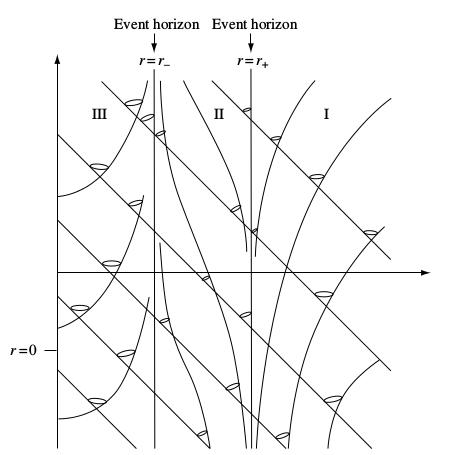
\includegraphics[width=0.8\textwidth]{conoluz.jpeg}
\caption{Espacio-tiempo en coordenadas de Eddington-Finkelstein donde se observan conoz de luz en la proximidad de los horizontes de eventos.}
\label{cono_foto}
\end{figure}

\begin{figure}[H]
\centering
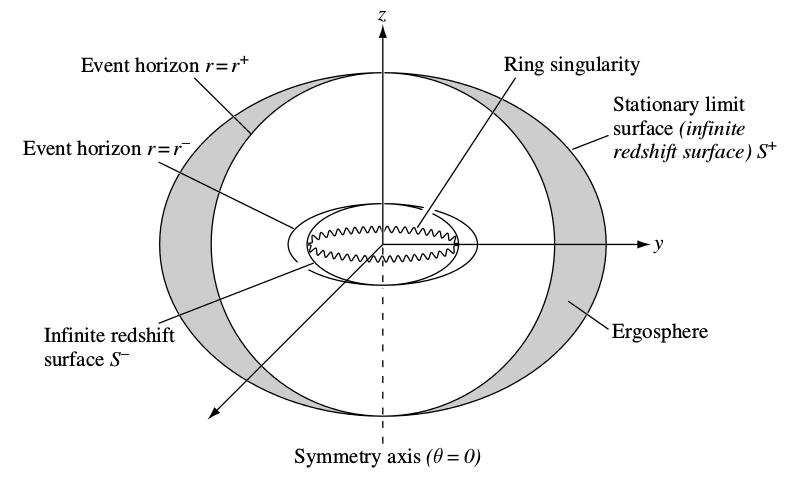
\includegraphics[width=\textwidth]{kerr.jpeg}
\caption{Diagrama del espacio alrededor de un agujero negro de Kerr. Donde se puede observar la singularidad tipo anillo, el horizonte de eventos y la ergosfera.}
\label{kerr_metric}
\end{figure}

%-----AGUJEROS-NEGROS-EXTREMOS-Y-SINGULARIDADES-DESNUDAS---------------------
\subsection{Agujeros negros extremos y Singularidades desnudas}\label{ebh}
En el caso donde un agujero negro posea un momento angular tal que $J=M^2$ los horizontes de eventos \ref{horeventos} pasan a solaparse y definir una región $r_{\pm}=\mu$.

En 1969 Penrose postuló \cite{cosmiccensor} la \textit{hipótesis de censura cósmica} que dice que no existen singularidades desnudas ya que todas las singularidades deben estar ocultas detrás de un horizonte de eventos.
Para el caso $a^2>\mu ^2$ se encuentra que ahora $\Delta =0$ no se sigue satisfaciendo, es más $\Delta >0$ en todo el espacio. Esto tiene como consecuencia que no existen los horizontes de eventos. Pero la singularidad en $\rho =0$ sigue prevaleciendo. Éste fenómeno es llamado \textbf{Singularidad desnuda}. La existencia de la misma implicaría que la misma fuera vista por cualquier observador, pero dicho problema no es estudiado por la hipótesis propuesta por Penrose.


 \section{Agujeros negros astrofísicos}
Dado que un agujero negro no emite radiación más que la hipotética radiación de Hawking su identificacióm se suele hacer de manera indirecta. Con el objetivo de detectar la radiación de Hawking, el 11 de junio de 2008 la NASA junto con el departamente de energía de los Estados Unidos envío el telescopio de rayos gama Fermi también conocido por sus siglas GLAST (Gamma-Ray Large Area Space Telescope) \ref{fermi_foto} pero no pudo detectar esta señal hasta el momento \cite{fermi}. Aunque su misión no fue completamente fallida porque permitió hacer muchos otros descubrimientos en la astrofísica de altas energías.

\begin{figure}[H]
\centering
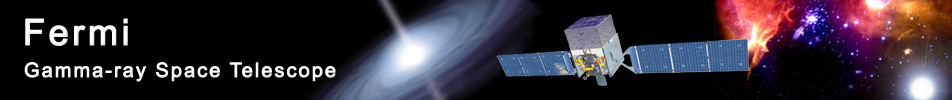
\includegraphics[width=\textwidth]{fermi_banner.jpg}
\caption{Imágen ilustrativa de la misión GLAST que tiene entre otros objetivos detectar la radiación de Hawking.}
\label{fermi_foto}
\end{figure}

La detección de agujeros negros de manera indirecta fue mucho más fructífera en lo que respecta a resultados. Las mismas se realizan debido a la interacción con la materia circundante con el agujero negro por ejemplo, como así también midiendo las ondas gravitacionales que generan.

En lo que respecta a estas últimas LIGO (Laser Interferometer Gravitational-Wave Observatory) \cite{ligo} intentó medir sin los resultados esperados ondas gravitacionales provocadas por agujeros negros. El mismo operó desde 2002 hasta 2010, pero se esperá que en un futuro cercano hayan nuevos instrumentos dedicadados a la medición de estas ondas, como es el caso de Advanced LIGO, LIGO-INDIA o Virgo, este último en Italia.

Se cree que un posible candidato a agujero negro es el que se encuentras en el centro de nuestra galaxia, llamado \textit{Sagitario A*}. Esto se logró monitoreando durante dos décadas las órbitas de 20 estrellas cercanas al centro en el infrarrojo. El periodo orbital de las mismas suele ser del orden de la vida humana, a excepción de una estrella que tiene un período de 11.5 años llamada \textit{S0-2}. Los resultados se muestran en la figura \ref{sgtaa} . Este estudió arrojó hasta el momento un valor de la masa estimada de agujero negro de $M=(4.4 \pm 0.27)\times 10^6 M_{\odot}$ la cual implicaría casi con seguridad la presencia de un agujero negro.

\begin{figure}[H]
\centering
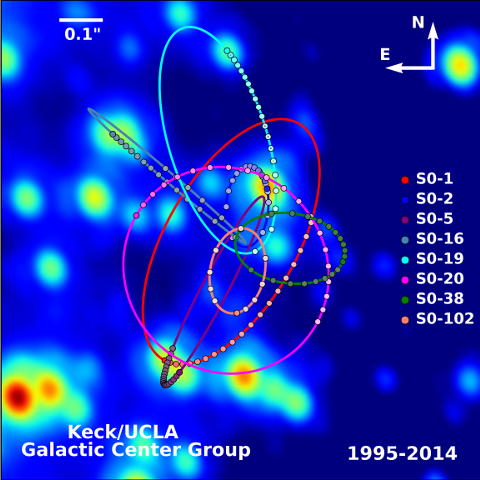
\includegraphics[width=0.7\textwidth]{sgta.jpg}
\caption{Trayectorias de las estrellas alrededor del agujero negro del centro de nuestra galaxia.}
\label{sgtaa}
\end{figure}

A su vez es posible medir la velocidad de rotación del agujero negro. La primera vez que se logró este objetivo  fue en el año 2013 por la misión NuStar (Nuclear Spectroscopic Telescope Array) \cite{nustar} de la NASA midiendo la emisión de rayos-X de un agujero negro disco de su disco de acreción. El resultado obtenido para el agujero negro en la galaxia NGC 1365 fue de $84\%$ el valor de la velocidad de la luz \cite{spin} . 

\begin{figure}[H]
\centering
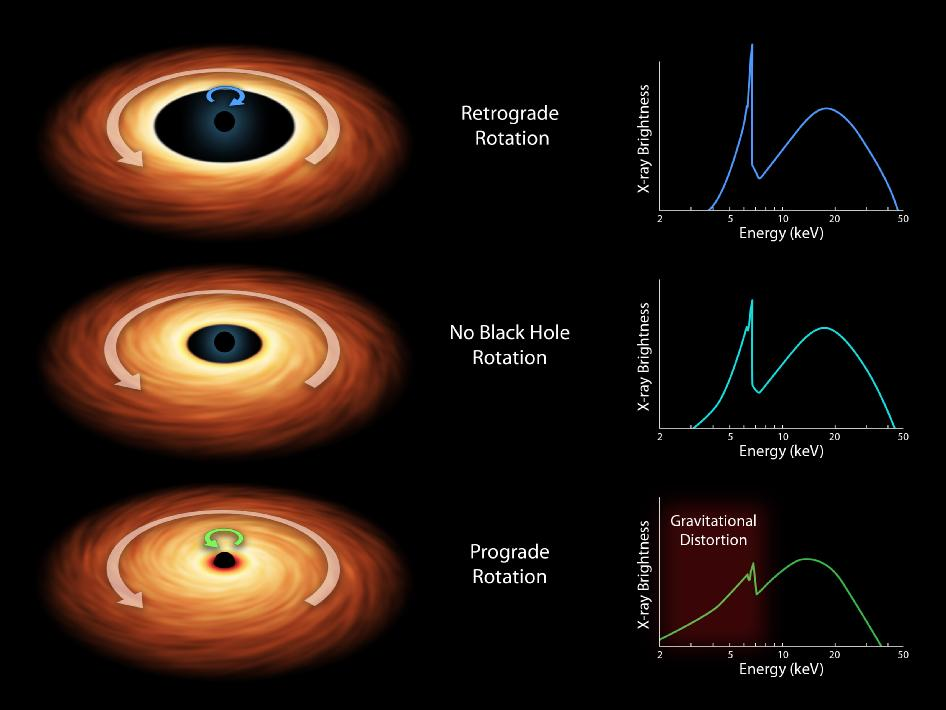
\includegraphics[width=0.7\textwidth]{spin_bh.jpg}
\caption{Señal esperada al observar la radiación en X proveniente de un agujero negro de acuerdo al sentido de rotación entre el disco de acreción y el agujero negro.}
\label{spin_bhh}
\end{figure}

A su vez, investigación reciente \cite{ehorizon} propone observar un horizonte de eventos de un agujero negro. Los agujeros negros son los únicos objetos que pueden tener un horizonte de eventos. Por lo tanto, la evidencia reafirma la existencia de estos. La idea es observar una sombra alrededor del agujero negro debido a la luz que se curva. Este efecto es independiente de la orientación y la velocidad de rotación del agujero negro. La teoría predice que la sombra debería estar centrada, pero en el caso de ser incorrecto el teorema del no-hair la sombra estaría dispersada hacia la derecha o izquierda \ref{ehbh_foto} .

\begin{figure}[H]
\centering
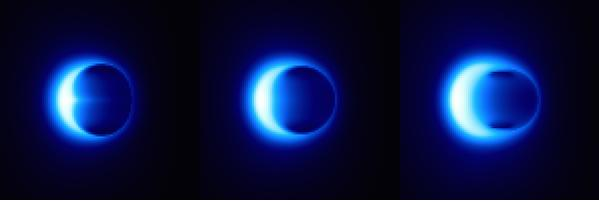
\includegraphics[width=0.7\textwidth]{ehbh.jpeg}
\caption{Observación del horizonte de eventos de un agujero negro. Se espera que la sombra del horizonte esté centrada alrededor del agujero negro si el teorema de no-hair es válido, sino la sombre se verá corrida hacia los costados.}
\label{ehbh_foto}
\end{figure}


\begin{thebibliography}{50}
\bibitem{wald} Wald, Robert M. General relativity. University of Chicago press, 2010.
\bibitem{kerr_paper}Kerr, Roy P. "Gravitational field of a spinning mass as an example of algebraically special metrics." Physical review letters 11.5 (1963): 237.
\bibitem{ph_sing}Penrose, Roger. "Gravitational collapse and space-time singularities." Physical Review Letters 14.3 (1965): 57-59.
\bibitem{hartle} Hartle, James B. Gravity: An introduction to Einstein's general relativity. Vol. 1. 2003.
\bibitem{cosmiccensor} Penrose, Roger. "The question of cosmic censorship." Journal of Astrophysics and Astronomy 20.3-4 (1999): 233-248.
\bibitem{matintro} Casadio, Roberto, et al. "A mathematical introduction to Kerr black holes."
\bibitem{fermi} Bains, Jagdev. "Searching for Evaporating Primordial Black Holes using Fermi Gamma Ray Telescope Data." (2011).
\bibitem{ligo} \url{http://www.ligo.caltech.edu/}
\bibitem{nustar} \url{http://www.nustar.caltech.edu/}
\bibitem{spin} Risaliti, G., et al. "A rapidly spinning supermassive black hole at the centre of NGC [thinsp] 1365." Nature 494.7438 (2013): 449-451.
\bibitem{ehorizon} Falcke, Heino, Fulvio Melia, and Eric Agol. "Viewing the shadow of the black hole at the galactic center." The Astrophysical Journal Letters 528.1 (2000): L13.
\end{thebibliography}



\end{document}


